% !TeX root = ../defense.tex

\section{Sustainable model use}
\frame{\sectionpage}

\begin{frame}{Optimisation model workflow}
    \begin{center}
    \begin{tikzpicture}[node distance=1.2cm and .75cm,font=\small]
        \setlength{\leftmargini}{10pt}

        \uncover<3->{%
            \node[flowbox] (data) {%
            \fbtitle{Data}\vphantom{yÖ}
            \nodepart{two}
            \begin{minipage}{.17\textwidth}
            \begin{itemize}\itemsep0em
            \item Tabular
            \item Geographic
            \item Database
            \end{itemize}
            \end{minipage}};
        }

        \uncover<1->{%
            \node[concept,above=of data,align=center,yshift=-.6cm] (question) {Research question};
        }
        \uncover<3->{\draw[conn] (question) -- (data);}

        \uncover<5->{%
            \node[flowbox,right=of data,onslide=<8->{fb-highlight}] (proc) {%
            \fbtitle{Processing}\vphantom{yÖ}
            \nodepart{two}
            \begin{minipage}{.17\textwidth}
            \begin{itemize}\itemsep0em
            \item MATLAB
            \item Python
            \item Excel
            \end{itemize}
            \end{minipage}};

            \draw[conn] (data) -- (proc);
        }

        \uncover<4->{%
            \node[flowbox,right=of proc] (model) {%
            \fbtitle{Model}\vphantom{yÖ}
            \nodepart{two}
            \begin{minipage}{.17\textwidth}
            \begin{itemize}\itemsep0em
            \item GAMS
            \item Pyomo
            \item YALMIP
            \end{itemize}
            \end{minipage}};
        }

        \uncover<5->{%
            \draw[conn] (proc) -- (model);
        }

        \uncover<6->{%
            \node[flowbox,right=of model] (solver) {%
            \fbtitle{Solver}\vphantom{yÖ}
            \nodepart{two}
            \begin{minipage}{.17\textwidth}
            \begin{itemize}\itemsep0em
            \item CPLEX
            \item Gurobi
            \item GLPK
            \end{itemize}
            \end{minipage}};

            \draw[conn] (model) -- (solver);
        }

        \uncover<7->{%
            \node[flowbox,below=of proc] (output) {%
            \fbtitle{Result}\vphantom{yÖ}
            \nodepart{two}
            \begin{minipage}{.17\textwidth}
            \begin{itemize}\itemsep0pt
            \item Reports
            \item Diagrams
            \item Maps
            \end{itemize}
            \end{minipage}};
        }

        % concept text nodes
        \uncover<2->{%
            \node[concept,above=of model,align=center,yshift=-.6cm] (assump) {Modelling assumptions};
            \draw[hidden] (question.east |- assump) --
                        node[below,text=tumdarkgrey,font=\itshape\scriptsize] {informs}
                        (assump);
        }

        \uncover<4->{%
            \draw[conn] (assump) -- (model);
        }

        \uncover<9->{%
            \node[concept,text height=1.5ex] at (output.east -| model.south) (interpret) {Interpretation};
            \draw[conn] (output) -- (interpret);
        }

        % connections
        \uncover<8->{%
            \draw[conn] (solver.south) -- ++(0,-.6cm) -|
                        node[below,near start] {Raw results}
                        (proc.290);
            \draw[conn] (proc.250) -- (output.north -| proc.250);
        }
        \uncover<10->{%
            \draw[conn] (output) -|
                        node[below,near start,anchor=north east] {Feedback}
                        (data);
        }
    \end{tikzpicture}
    \end{center}
\end{frame}

\begin{frame}{Distributed version control for scientific work}
    \begin{center}
    \begin{tikzpicture}[
            node distance=3em and 3em, pin distance=.75em,
            commit/.style={circle,fill=jdblue,draw=jddarkblue,inner sep=3pt},
            chain/.style={draw=jddarkblue,very thick},
            every pin/.style={draw=jdgreen,text=jdgreen},
            every pin edge/.style={draw=jdgreen},
            master/.style={fill=jdgreen!50,draw=jdgreen},
            summary/.style={anchor=west}
            ]

        \node[commit,onslide=<1>{master,pin=right:01.12.}] (origin) {};

        \uncover<2->{%
        \node[commit,right=of origin,onslide=<2>{master,pin=right:02.12.}] (c1) {};
            \draw[chain] (origin) -- (c1);}

        \uncover<3->{%
        \node[commit,right=of c1,onslide=<3-4>{master,pin=right:\ttfamily v1}] (c2) {};
            \draw[chain] (c1) -- (c2);}

        \uncover<4->{%
        \node[commit,below right=of c2,pin=below:\ttfamily haag15] (fork) {};
            \draw[chain] (c1) -- (c2 |- fork) -- (fork);}

        \uncover<5->{%
        \node[commit,right=4.5em of c2,onslide=<5>{master,pin=below:04.12.}] (c3) {};
            \draw[chain] (c2) -- (c3);
        \node[commit,above right=3em and 6em of c2,pin=above:\ttfamily feature] (feature) {};
            \draw[chain] (c2) -- ($(feature) - (3em, 0)$) -- (feature);}

        \uncover<6->{%
        \node[commit,below right=of feature,onslide=<6->{master},
              pin=below:\ttfamily v3] (merge) {};
            \draw[chain] (feature) -- (merge);
            \draw[chain] (c3) -- (merge);}

        \uncover<7->{%
        \node[right=4em of merge,summary] (devel) {Development};
        \node[summary] (collab) at (feature -| devel.west) {Collaboration};
        \node[summary] (archiv) at (fork -| devel.west) {Archival};
        }

    \end{tikzpicture}
    \end{center}
\end{frame}

\fullframegraphic{img/urbs/urbs-commit-network-transp}

\begin{frame}{Conclusion}
    \begin{center}
    \begin{tikzpicture}[node distance=1em and 2ex,font=\small]
        \node[flowbox,fb-muted] (infra) {
            \fbtitle{Infrastructure}\vphantom{yÖ}
        \nodepart{two}
            \begin{minipage}{.29\textwidth}
                \centering
                \vspace{3.3ex}
                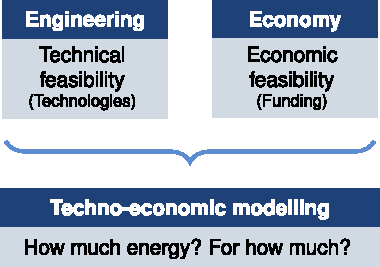
\includegraphics[width=.98\textwidth]{img/techno-economic-modelling}
                \vspace{3.3ex}
            \end{minipage}
        };

        \node[flowbox,fb-muted,right=of infra] (model) {
            \fbtitle{Modelling}\vphantom{yÖ}
        \nodepart{two}
            \begin{minipage}{.29\textwidth}
                \centering
                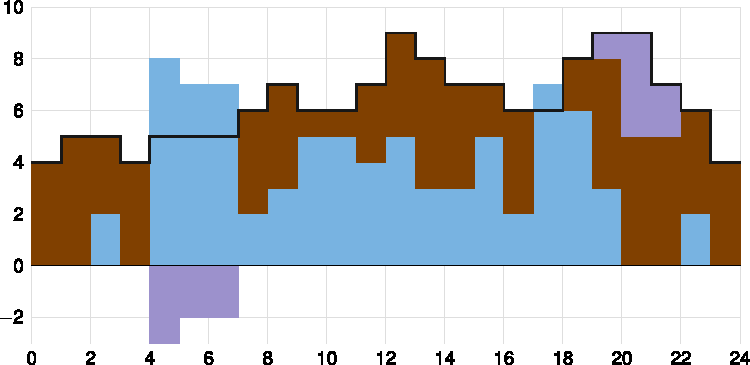
\includegraphics[width=.95\textwidth]{img/urbs/urbs-ts-graph}
                \vspace{2ex}
                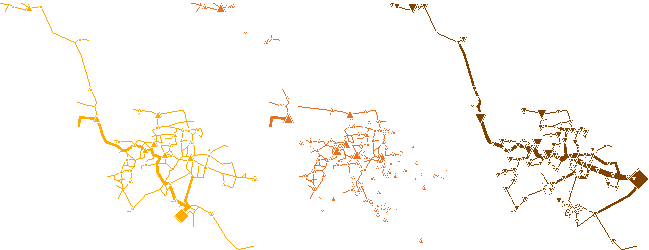
\includegraphics[width=.95\textwidth]{img/rivus/scen-today-rivus-networks}
                \vspace{1ex}
            \end{minipage}
        };

        \node[flowbox,fb-muted,right=of model] (open) {
            \fbtitle{Open Source}\vphantom{yÖ}
        \nodepart{two}
            \begin{minipage}{.29\textwidth}\raggedright
                \centering
                \vspace{2.9ex}
                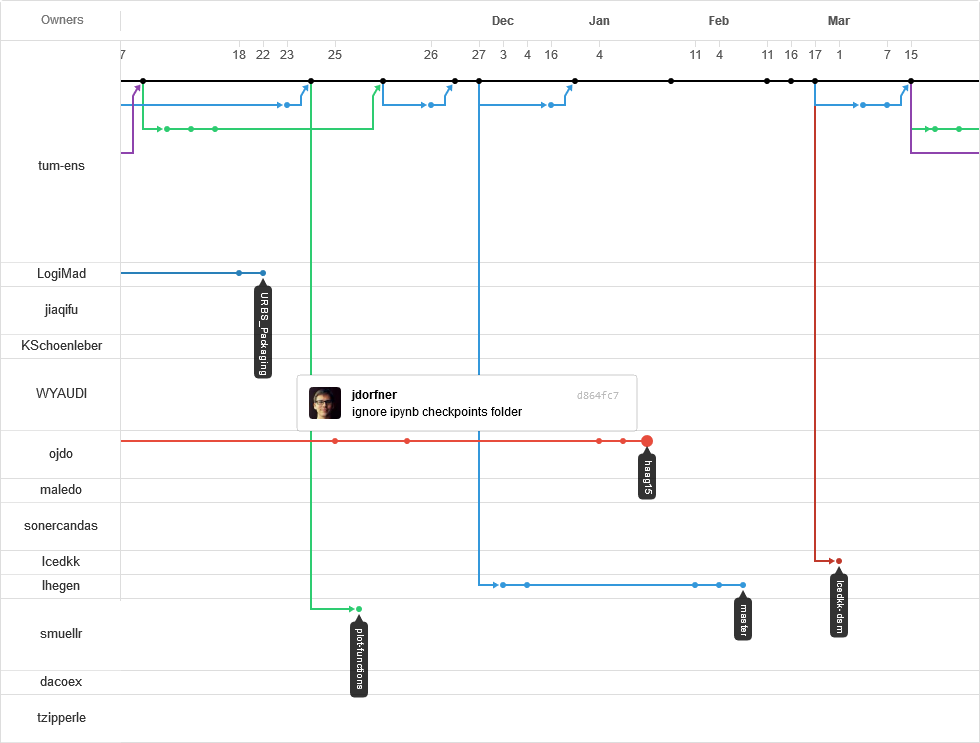
\includegraphics[width=.95\textwidth]{img/urbs/urbs-commit-network-transp}
                \vspace{2.9ex}
            \end{minipage}
        };
    \end{tikzpicture}
    \end{center}
\end{frame}
